\chapter{Future Work} \label{fw}

This chapter will outline a plan for future work and relates back to our research questions chapter. \ref{rq}

We will look at feature extraction for systematic reviews. This will involve looking at content within a study and attempting to identify it automatically. The first step of this process is being able to obtain relevant studies for a systematic review. We will look at techniques for obtaining these in the form of pdf files. Work will also need undertaking in processing a diverse range of pdf documents. We will will then need to look at bringing in annotators to mark when the relevant information occurs with a study, or look for common patterns that occur across all studies. This is likely to be a very challenging, but potentially very beneficial task. We would also like to apply an approach to PICO extraction from studies. We would like to expand upon the existing work \ref{picoExtr} from abstract-level extraction to document level extraction.


We will investigate classification of studies and determine if we can make a binary decision on whether or not a study is relevant to a research question. To achieve this we will first need to process the content of the studies and decide on a sampling strategy. This might involve using a proportion of the relevant studies as a training examples, and then trying to classify the remainder of the studies. We will also look at using unsupervised methods, by trying to directly use the systematic review as an indicator of relevant studies. We will need to overcome the challenge of condensing large studies (e.g full pdf texts) into relevant chunks.


Finally we will look at alternate approaches to finding stopping points. We found both our sampling methods \ref{samplemethods} were getting beat by our baseline methods \ref{baselineapp}. As such, we should look into alternate regression-based techniques for the sample methods.

\section{Gnatt Chart}

\begin{sidewaysfigure}


\begin{figure}[H]
\center
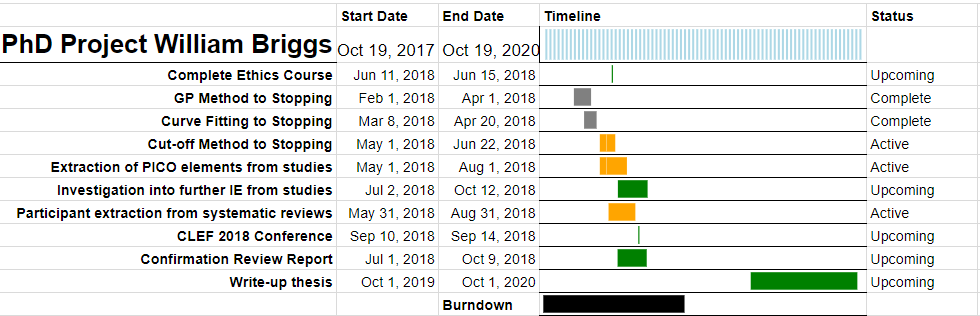
\includegraphics[height=7cm]{figures/gnatt.png}
\caption{Gnatt Chart}
\end{figure}
\end{sidewaysfigure}


